\documentclass[tikz,border=6pt]{standalone}
\usepackage{tikz}
\usepackage{amsmath,amssymb}
\usetikzlibrary{shapes.geometric, arrows.meta, positioning}

\definecolor{hbmorange}{RGB}{230,136,28}
\definecolor{smgreen}{RGB}{44,160,44}
\definecolor{regblue}{RGB}{70,130,180}
\definecolor{accentred}{RGB}{214,39,40}
\definecolor{choice}{RGB}{240,210,60}

\begin{document}
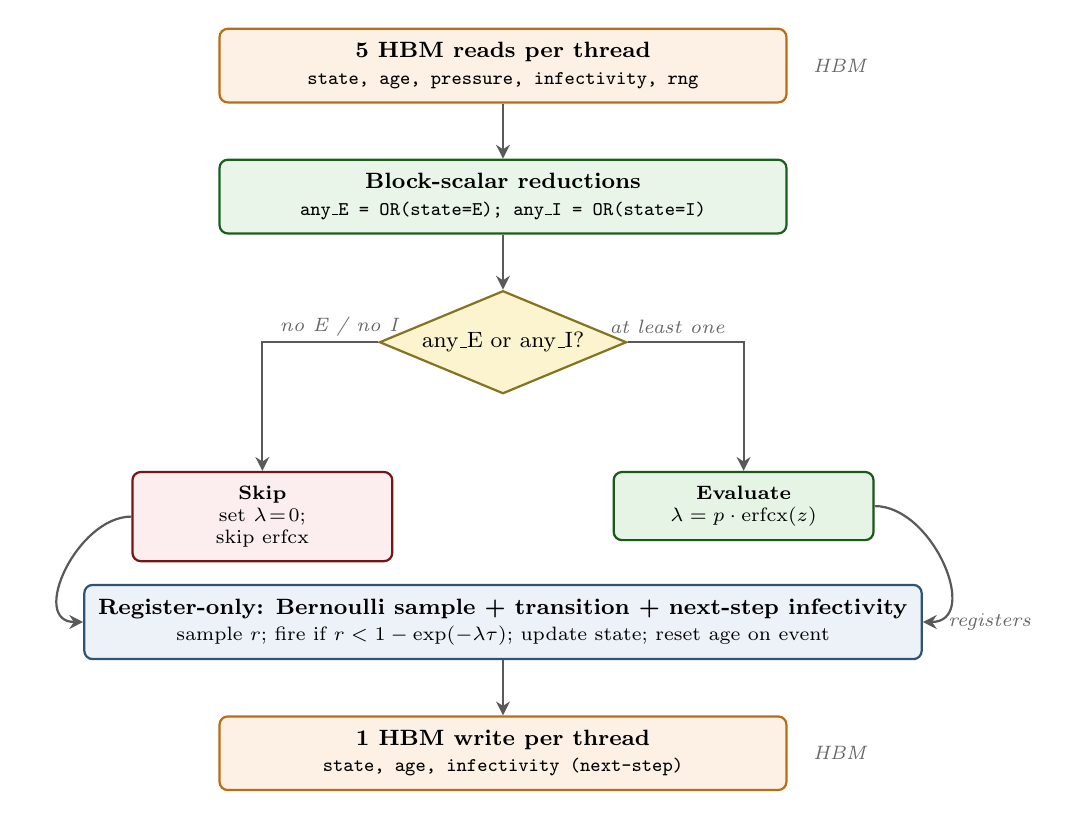
\begin{tikzpicture}[
    node distance=7mm and 5mm,
    box/.style={rectangle, rounded corners=3pt, draw, align=center,
                font=\footnotesize, inner sep=5pt, line width=0.8pt},
    hbmbox/.style={box, draw=hbmorange!80!black, fill=hbmorange!12,
                   minimum width=7.2cm},
    scalarbox/.style={box, draw=smgreen!60!black, fill=smgreen!10,
                      minimum width=7.2cm},
    regbox/.style={box, draw=regblue!65!black, fill=regblue!10,
                   minimum width=9.0cm},
    decision/.style={diamond, draw=choice!55!black, fill=choice!25,
                     aspect=2.4, inner sep=2pt, font=\footnotesize,
                     align=center, line width=0.8pt},
    skipbox/.style={box, draw=accentred!55!black, fill=accentred!8,
                    minimum width=3.3cm, font=\scriptsize},
    evalbox/.style={box, draw=smgreen!55!black, fill=smgreen!12,
                    minimum width=3.3cm, font=\scriptsize},
    flow/.style={-{Stealth[length=5pt,width=5pt]}, line width=0.8pt,
                 color=black!65},
    lbl/.style={font=\scriptsize\itshape, text=black!60},
]

\node[hbmbox] (reads)
     {\textbf{5 HBM reads per thread}\\
      \texttt{\scriptsize state, age, pressure, infectivity, rng}};

\node[scalarbox, below=of reads] (scalar)
     {\textbf{Block-scalar reductions}\\
      \texttt{\scriptsize any\_E = OR(state=E);\ any\_I = OR(state=I)}};

\node[decision, below=of scalar] (dec) {any\_E or any\_I?};

\node[skipbox, below left=13mm and 6mm of dec] (skip)
     {\textbf{Skip}\\set $\lambda\!=\!0$;\\
      skip erfcx};

\node[evalbox, below right=13mm and 6mm of dec] (eval)
     {\textbf{Evaluate}\\$\lambda = p \cdot \mathrm{erfcx}(z)$};

\node[regbox, below=24mm of dec] (bern)
     {\textbf{Register-only: Bernoulli sample + transition + next-step infectivity}\\
      \scriptsize sample $r$;\ fire if $r < 1 - \exp(-\lambda \tau)$;\ update state; reset age on event};

\node[hbmbox, below=of bern] (write)
     {\textbf{1 HBM write per thread}\\
      \texttt{\scriptsize state, age, infectivity (next-step)}};

\draw[flow] (reads) -- (scalar);
\draw[flow] (scalar) -- (dec);
\draw[flow] (dec.west) -| (skip.north);
\draw[flow] (dec.east) -| (eval.north);
% Route the skip and evaluate exits around the OUTSIDE of the
% figure (west-to-west, east-to-east) so the arrows do not cross
% the central axis or overlap the decision block. This matches the
% cleaner left-and-right merge pattern used in other block diagrams
% in the manuscript.
\draw[flow] (skip.west) to[out=180, in=180, looseness=1.2] (bern.west);
\draw[flow] (eval.east) to[out=0, in=0, looseness=1.2] (bern.east);
\draw[flow] (bern) -- (write);

\node[lbl] at ([yshift=2mm, xshift=-5mm] dec.west) {no E / no I};
\node[lbl] at ([yshift=2mm, xshift=5mm] dec.east) {at least one};

\node[lbl, right=2mm of reads] {HBM};
\node[lbl, right=2mm of bern] {registers};
\node[lbl, right=2mm of write] {HBM};

\end{tikzpicture}
\end{document}
